\documentclass[
  11pt,
  letterpaper,
   addpoints,
   answers
  ]{exam}

\usepackage{../exercise-preamble}
\usepackage{multicol}
\begin{document}

\noindent
\begin{minipage}{0.47\textwidth}

\includegraphics[width=\textwidth]{../fcfm_die}
\end{minipage}
\begin{minipage}{0.53\textwidth}
    
\begin{center} 
\large\textbf{Análisis y Diseño de Circuitos Eléctricos} (EL3101-2) \\
\large\textbf{Clase auxiliar 5} \\
\normalsize Prof.~Santiago Bradford V.\\
\normalsize Prof.~Aux.~Erik Saez A. - Rodrigo Catalán\\
             - Byron Castro R.
\end{center}
\end{minipage}

\vspace{0.5cm}
\noindent
\vspace{.85cm}

\begin{center}
    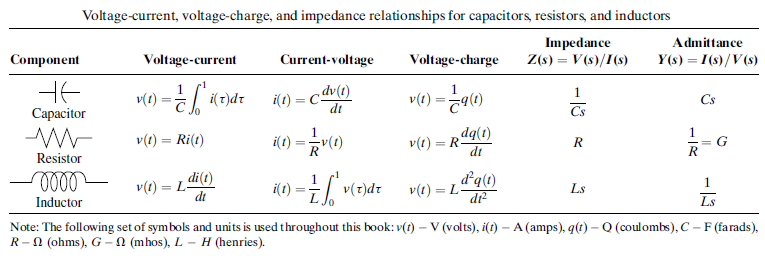
\includegraphics[width=0.9\textwidth]{Auxiliar_5_14}
    \captionof{figure}{Tabla resumen}
\end{center}

\begin{questions}
    %%%%%%%%%%%%%%%%%%%%%%%%%%%
    \question 
    El circuito de la figura 2 contiene interruptores que han estado abiertos por mucho tiempo. En \( t = 0\,[\text{s}] \) se cierra el interruptor de la derecha mientras que en \( t = 1\,[\text{s}] \) se cierra el de la izquierda. En base a la situación descrita, se pide que:
    \begin{center}
        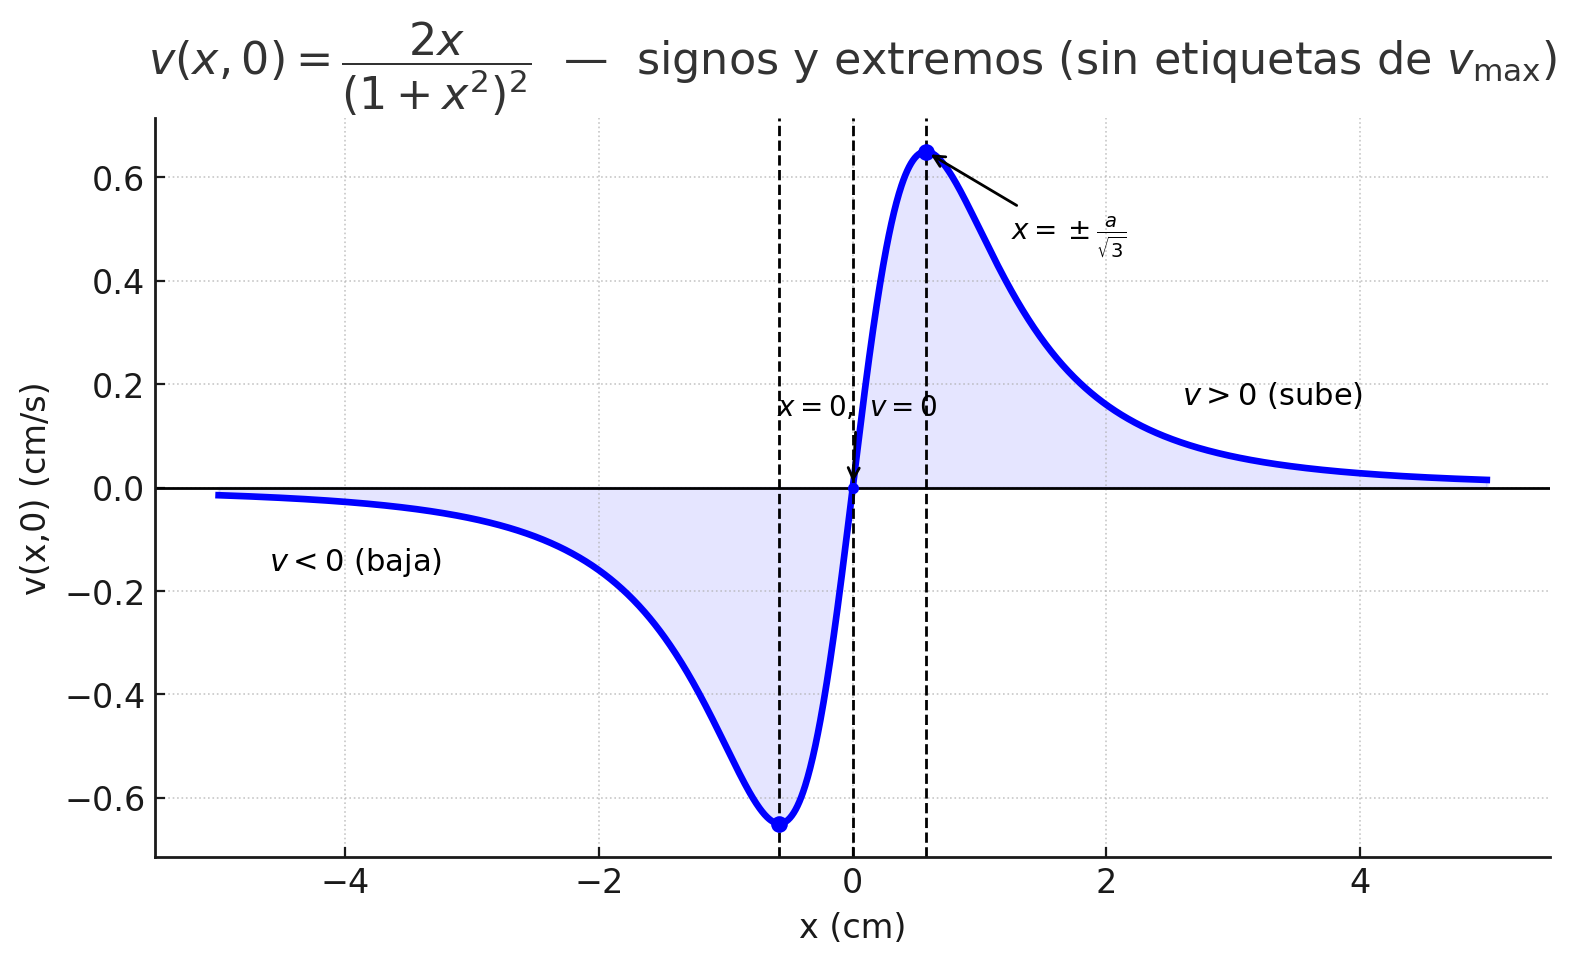
\includegraphics[width=0.45\textwidth]{Auxiliar_5_2}
        \captionof{figure}{Esquema del circuito}
    \end{center}

    \begin{enumerate}
        \item[a)] Determine \( v(t) \) para \( t > 0 \).
    
        \item[b)] Calcule la respuesta de entrada cero y respuesta cero de \( v(t) \) para \( t > 1 \).
    
        \item[c)] Calcule la energía que consume o suministra el condensador en el intervalo \( t \in [1, 1{,}5] \).
    \end{enumerate}
    %%%%%%%%%%%%%%%%%%%%%%%%%%%%
    \begin{solution}
        \begin{enumerate}
            \item Se busca obtener el voltaje $v(t)$ para $t > 0$, dado que el circuito presenta un condensador, este introducira una ecuacion diferencial de primer orden en el circuito, por lo que se debe obtener su condicion inicial, para esto se debe considerar el circuito en $t<0$ tenemos que:
            \begin{center}
                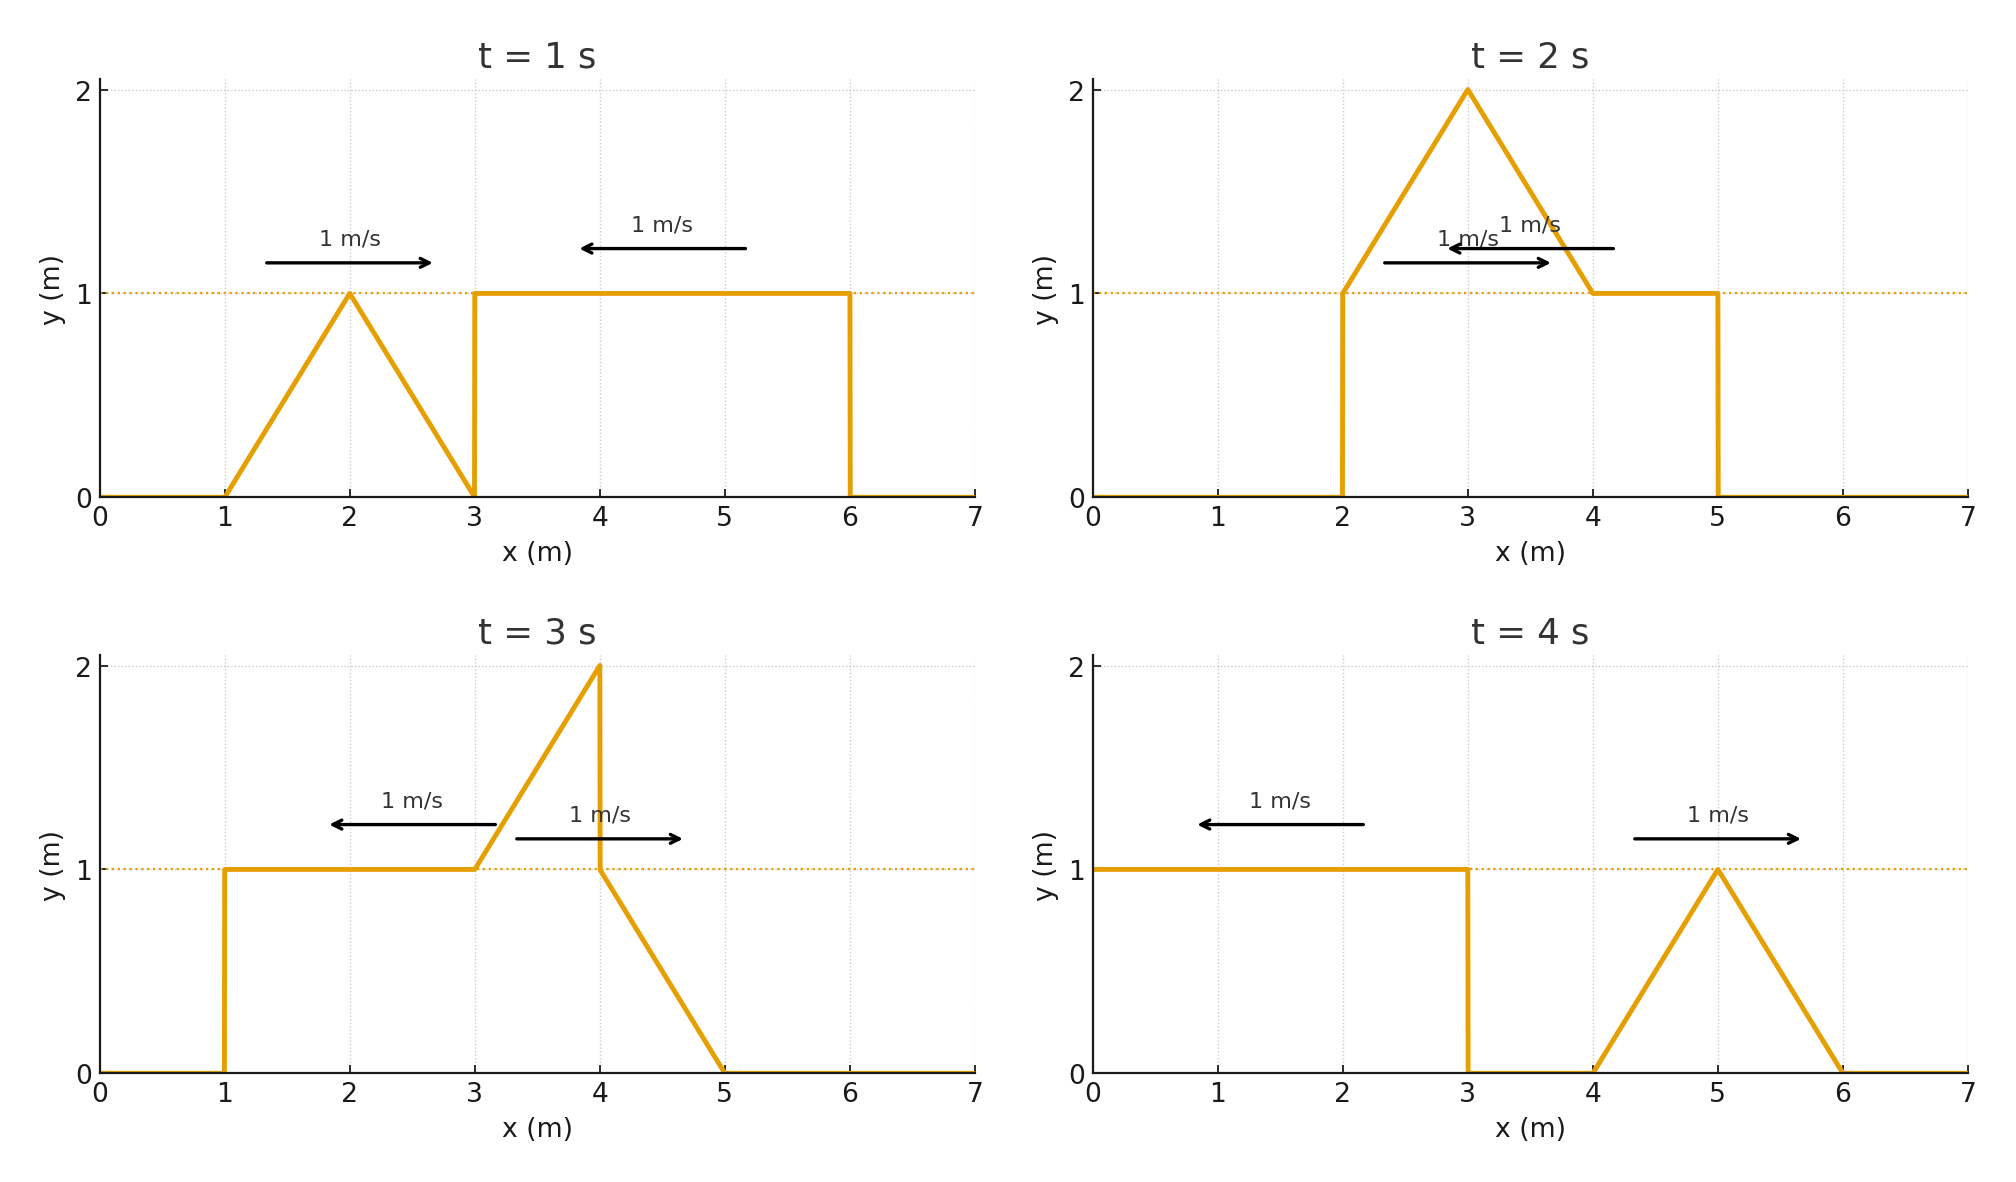
\includegraphics[width=0.3\textwidth]{Auxiliar_5_3}
                \captionof{figure}{Esquema del circuito para un tiempo $t<0$}
            \end{center}
            Se observa que para un tiempo $t<0$ el condensador se descargaria a tierra, por lo que es posible considerar que:
            $V_{c}(t=0^{-})=0$, luego tenemos que:
            \begin{center}
                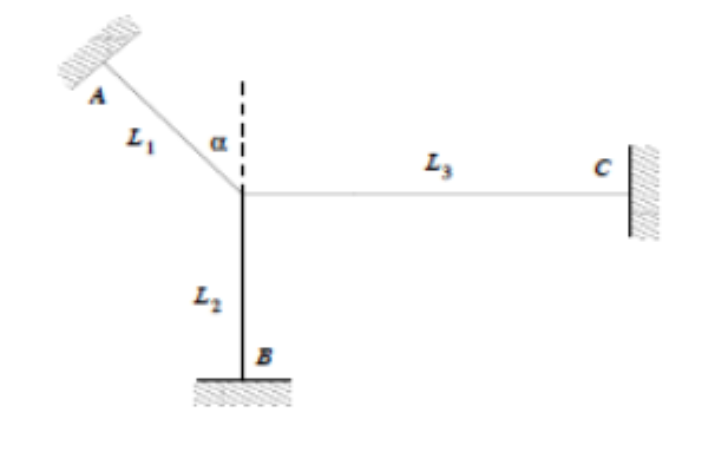
\includegraphics[width=0.35\textwidth]{Auxiliar_5_4}
                \captionof{figure}{Esquema del circuito para un tiempo $0<t<1$}
            \end{center}
            De esta manera se tiene que realizando mallas se obtiene que:
            \begin{align}
                \text{Malla 1:} \quad & I_1 \cdot 2\,\Omega + v + (I_1 - I_2) \cdot 8\,\Omega = 0 \\
                \text{Malla 2:} \quad & I_2 = 3\,\text{A}
            \end{align}
            Dado que la corriente en el condensador es $I_{1}$ y esta viene dada por $I_{1}= C \frac{\partial v}{\partial t}$ (Donde tenemos que C=0.1), por lo que las ecuaciones vendran dadas por:
            \begin{align}
                2 \cdot 0.1 \frac{\partial v}{\partial t} + v + (0.1 \cdot \frac{\partial v}{\partial t} - 3) \cdot 8 &= 0\\
                 \frac{\partial v}{\partial t} + v - 24 &= 0\\ 
            \end{align}
            Dada la propiedad de continuidad del potencial electrico, tendremos que se debe cumplir que $V(0^{-})=V(0)$, por lo que se tiene que resolviendo la EDO:
            \begin{align}
                v(t) = a_{1}e^{-t} + 24\\
            \end{align}
            Aplicando la condicion de borde 
            \begin{align}
                v(0) = 0 = a_{1} + 24\\
                a_{1} = -24
            \end{align}
            De esta manera tenemos que el voltaje v(t) sera de la forma:
            \begin{align}
                v(t) = -24e^{-t} + 24\\
                v(t) = 24(1-e^{-t})\\
            \end{align}
            Luego queremos analizar el siguiente caso:
            \begin{center}
                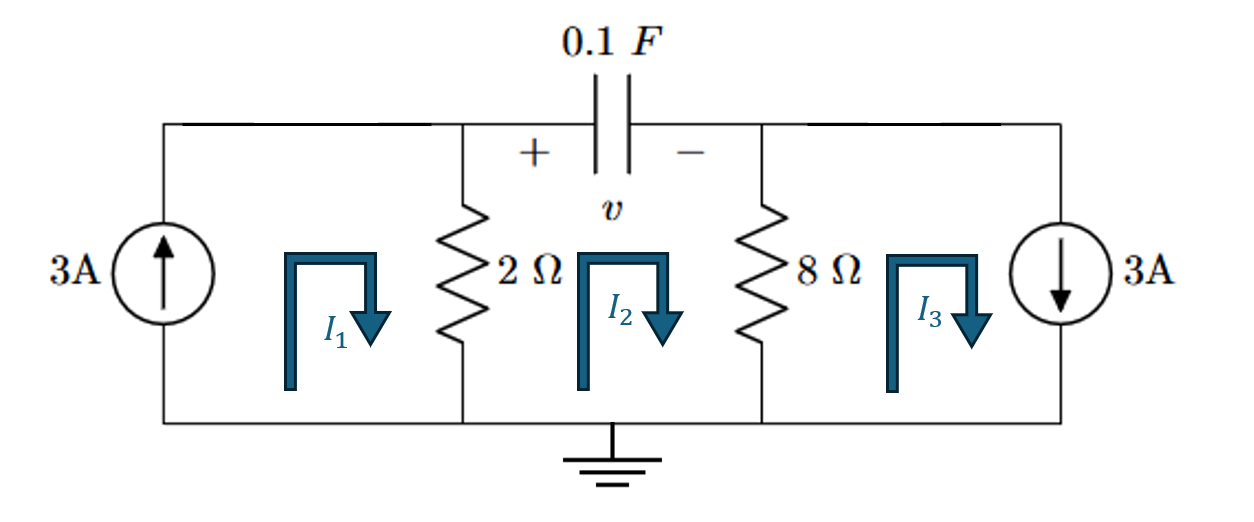
\includegraphics[width=0.45\textwidth]{Auxiliar_5_5}
                \captionof{figure}{Esquema del circuito para un tiempo $1<t<\infty$}
            \end{center}
            Luego tenemos que las mallas vendran dadas por las ecuaciones:
            \begin{align}
                \text{Malla 1:} \quad & I_1 =3\\
                \text{Malla 2:} \quad & 2(I_{2} - I_{1}) + v + 8(I_{2}- I_{3}) = 0 
                \\ 
                \text{Malla 3:} \quad & I_3 = 3\
            \end{align}
            Al igual que el caso anterior tenemos que la corriente por el condensador sera 
            \begin{align}
                I_{c} = I_{2} = 0.1\frac{\partial v}{\partial t}
            \end{align}
            \begin{align}
                &2\left(0{,}1\,\frac{d v}{d t} - 3\right) + v + 8\left(0{,}1\,\frac{d v}{d t} - 3\right) = 0 \\
                &\frac{d v}{d t} + v - 30 = 0 
            \end{align}
            Luego resolviendo mediante TI, tenemos el siguiente resultado:
            \begin{align}
                v(t) = b e^{-t} + 30
            \end{align}
            Es importate que debemos ajustar esta funcion con un retraso de 1 segundo, debido a los intervalos del tiempo, es decir:
            \begin{align}
                v(t) = b e^{-(t-1)} + 30
            \end{align}
            Luego para obtener $b$ debemos aplicar la condicion de continuidad del voltaje, es decir $v(1^{-})=v(1^{+})$, por lo que usamos la ecuacion de voltaje obtenida con anterioridad:
            \begin{align}
                v(t) = 24(1-e^{-1})\\
                v(1) = 24(1-e^{-1}) = 15.17 
            \end{align}
            Luego usando este valor obtenido tenemo sque para b:
            \begin{align}
                v(1) = b e^{-(1-1)} + 30\\
                15.17 = b + 30\\
                b = -14.83
            \end{align}
            con lo que finalmente tenemos que:
            \begin{align}
                v(t) = 30 - 14.83 e^{-(t-1)}
            \end{align}
            con lo que finalmente tenemos que la solucion vendra dada por:
            \begin{equation}
                v(t) =
                \begin{cases}
                24\left(1 - e^{-t}\right), & 0 < t < 1 \\
                -14.8291\, e^{-(t-1)} + 30, & t \geq 1
                \end{cases}
                \end{equation}
            \item[b)] Se busca la respuesta de entrada cero y respuesta estado cero de $v(t)$ para $t > 1$. Para esto debemos recordar lo siguiente:
            \begin{itemize}
                \item \textbf{Respuesta de entrada cero:} Corresponde a la respuesta del circuito cuando las fuentes independientes se apagan, y se deben considerar las condiciones iniciales.
                \item \textbf{Respuesta de estado cero:} Corresponde a la respuesta del circuito frente a las entradas, pero las condiciones iniciales se consideran nulas.
            \end{itemize}
            La utilidad de esto, es que podemos obtener la respuesta total del circuito, como:
            \begin{equation}
                \text{Respuesta Total} = \text{Respuesta de entrada cero} + \text{Respuesta de estado cero}
            \end{equation}
            Comenzando con la respuesta a entrada cero, se deben apagar las fuentes de corrientes, es decir que:
            \begin{center}
                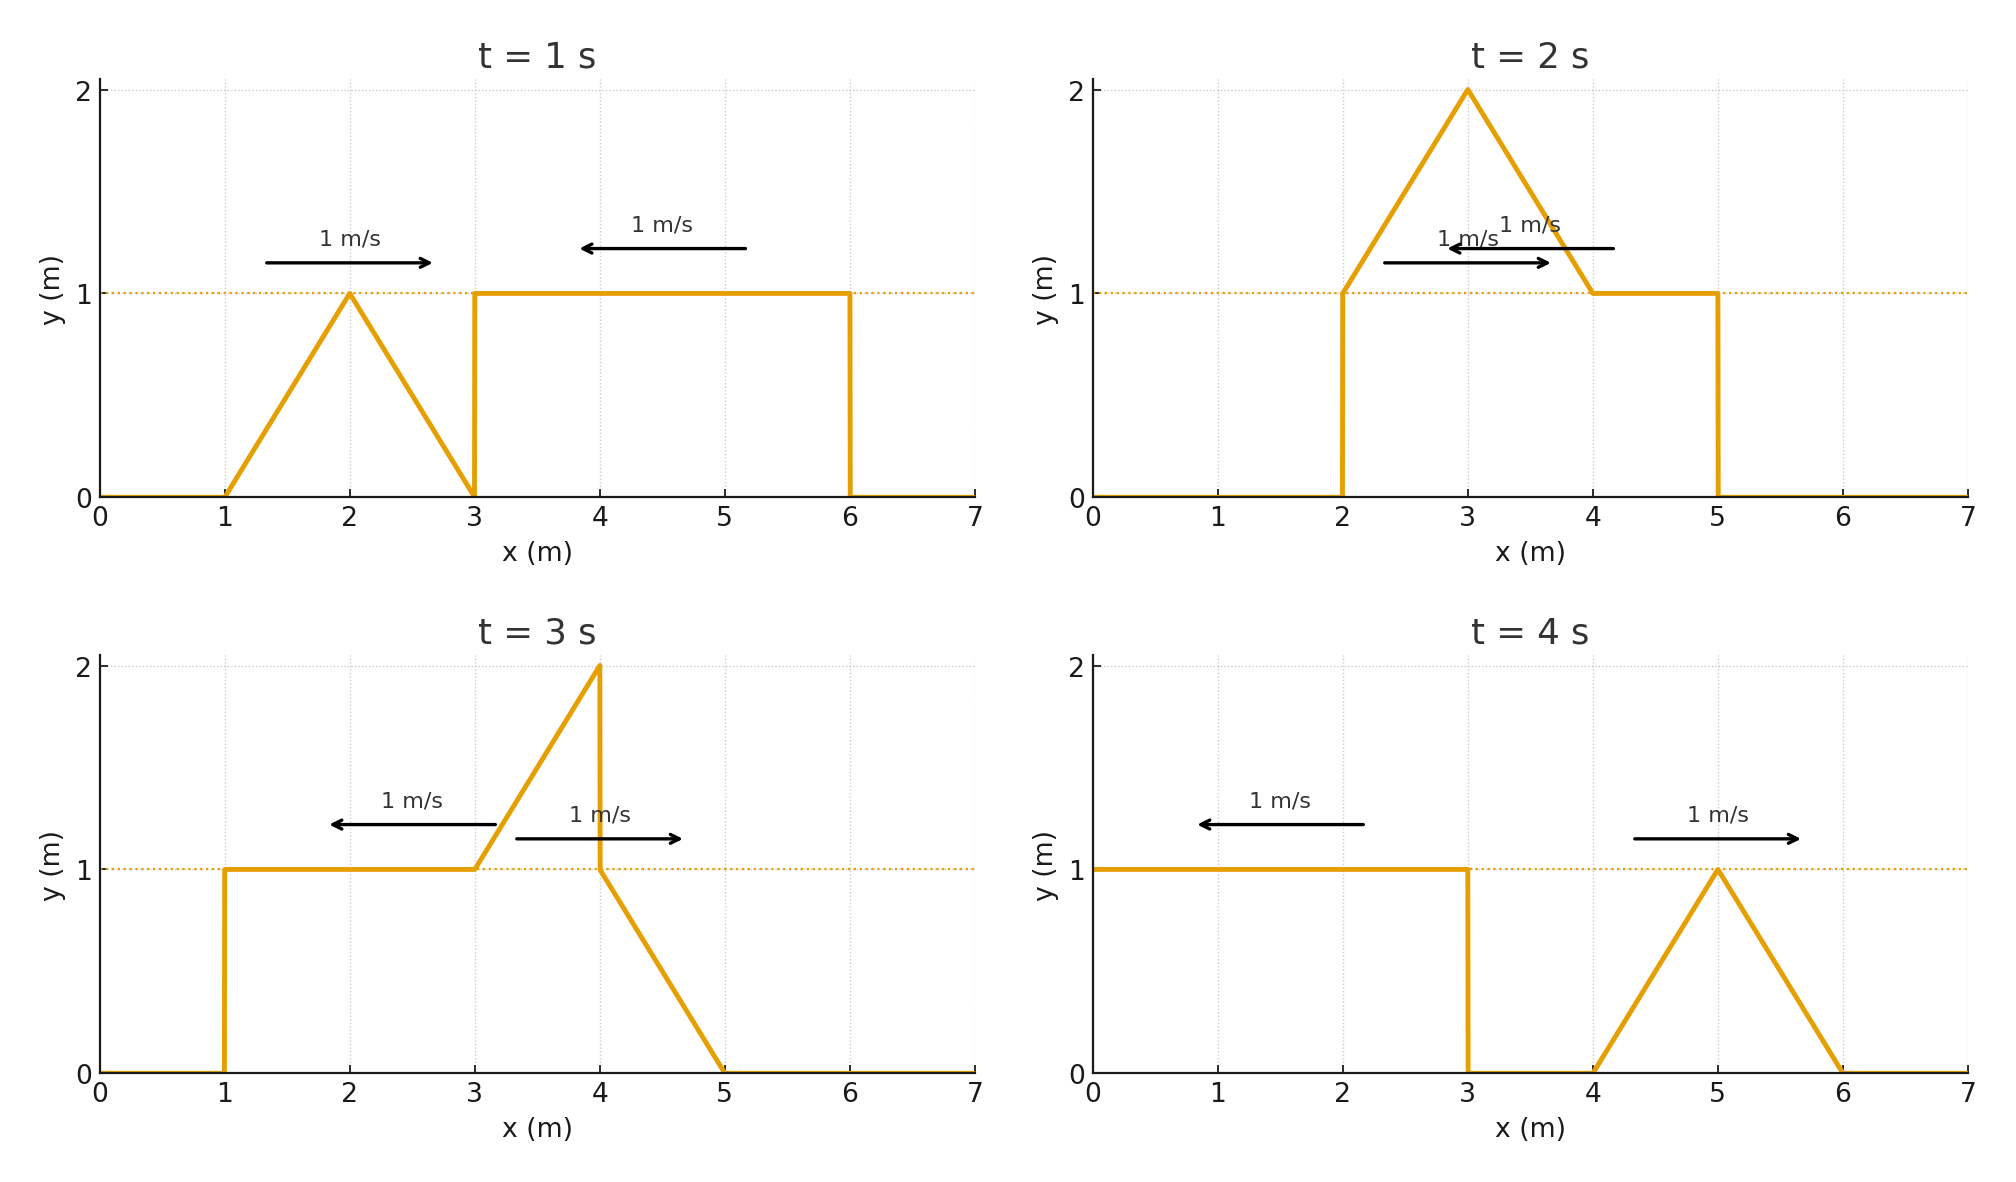
\includegraphics[width=0.25\textwidth]{Auxiliar_5_3}
                \captionof{figure}{Esquema del circuito para un tiempo para la RENC}
            \end{center}
            Luego realizando una malla, tenemos lo siguiente:
            \begin{align}
                v_{c} + 10i_{c} &= 0\\
                v_{c} + 10 \left(C \frac{\partial v_{c}}{dt}\right)&=0
            \end{align}
            Tenemos que la condicion inicial viene dada por $v_{c}(t=1) = 15.17$, por lo que tenemos finalmente que:
            \begin{align}
                v_{c}(t) = 15.1709e^{-(t-1)}
            \end{align}
            Por otro lado la respuesta de estado cero, se deben considerar las condiciones iniciales nulas, por lo que el circuito vendra dado por:
            \begin{center}
                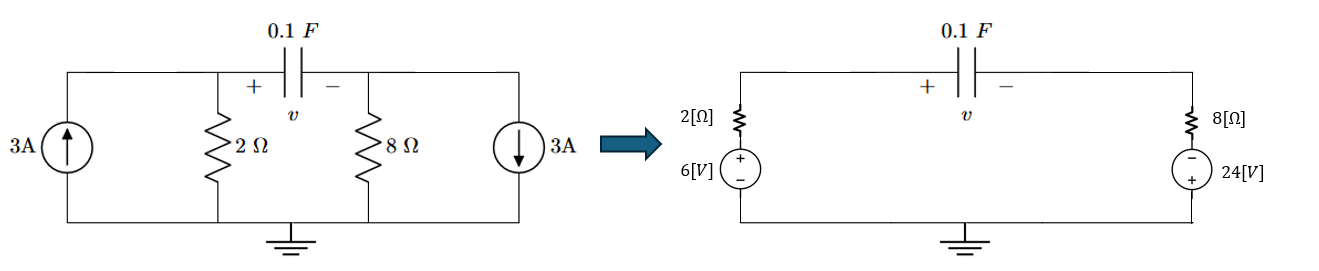
\includegraphics[width=0.7\textwidth]{Auxiliar_5_6}
                \captionof{figure}{Esquema del circuito para un tiempo para la RESC}
            \end{center}
            De esta manera tenemos que mediante una malla se obtiene que:
            \begin{align}
                -6 + 2i_{c} + v_{c} + 8i_{c}-  24 &= 0\\
                -6 + 10i_{c} + v_{c} &= 0\\
                v_{c} + 10 \left(C \frac{\partial v_{c}}{dt}\right)&=0
            \end{align}
            Dado que la condicion inicial viene dada por $v_{c}(t=1) = 0$, por lo que tenemos finalmente que:
            \begin{align}
                v_{c}(t) = 30(1-e^{-(t-1)}) 
            \end{align}
            Por lo que la respuesta total vendra dada por:
            \begin{align}
                v_{c}(t) = 15.1709e^{-(t-1)} + 30(1-e^{-(t-1)})
            \end{align}
            \item[c)] Se busca la energia que consume o suministra el condensador en el intervalo $t \in [1, 1{,}5]$, por lo que se considera que:
            \begin{align}
            E_{[1, 1.5]}= E(1.5) - E(1)
        \end{align}
            Recordando que la energia almacenada en un condensador es:
        \begin{equation}
            E = \frac{1}{2}C v^{2}
        \end{equation}
        Tenemos por tanto que:
        \begin{align}
            E_{[1, 1.5]} &= \frac{1}{2}C v^{2}(1.5) - \frac{1}{2}C v^{2}(1)\\
            =&9.2986[J]
        \end{align}
        Obteniendo la energia que consume el condensador en el intervalo $t \in [1, 1{,}5]$.
    \end{enumerate}
    \end{solution}
    %%%%%%%%%%%%%%%%%%%%%%%%%%%%
    \question

    Para el circuito de la figura  suponga que el interruptor ha estado en la posición \( a \) por mucho tiempo hasta que en \( t > 0 \) se conecta a \( b \).

\begin{enumerate}
    \item Determine \( i_1(0) \), \( i_2(0) \), \( v_0(0) \) y \( i_L(0) \).
    
    \item Si se conecta una fuente de corriente \( i_m(t > 0) = e^{\frac{1}{2}t} \) en paralelo y conservando la polaridad de \( v_0 \) justo en \( t = 0 \). Calcular la RESC.
    
    \item Calcule la RENC del caso anterior.
    
    \item Determine la respuesta completa del circuito.
    
    \item Determine \( i_L(\infty) \). ¿Tiene sentido su resultado?
    
    \item Determine \( i_1(\infty) \), \( i_2(\infty) \), \( v_0(\infty) \).
\end{enumerate}
\begin{center}
    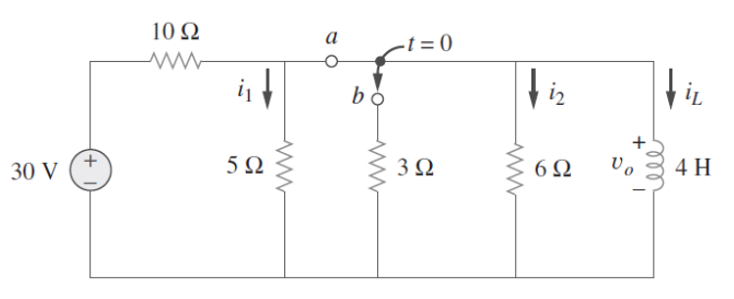
\includegraphics[width=0.6\textwidth]{Auxiliar_5_10}
    \captionof{figure}{Esquema del circuito para un tiempo $t<0$}
\end{center}
%%%%%%%%%%%%%%%%%%%%%%%%%%%%%
\begin{solution}
    \begin{enumerate}
        \item Se busca obtener los valores iniciales de $i_{1}(0)$, $i_{2}(0)$, $v_{0}(0)$ y $i_{L}(0)$, por lo que se debe considerar el circuito para un tiempo $t<0$, es decir:
        \begin{center}
            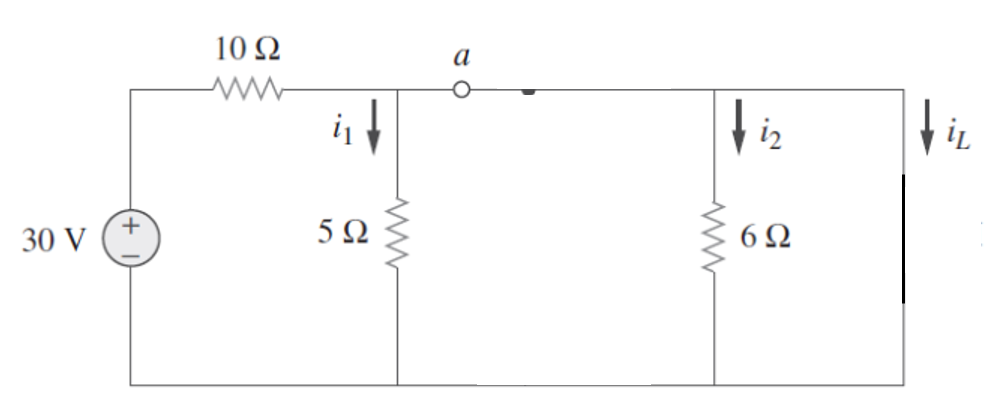
\includegraphics[width=0.6\textwidth]{Auxiliar_5_7}
            \captionof{figure}{Esquema del circuito para un tiempo $t<0$}
        \end{center}
        Tenemos que la inductancia se comporta como un cortocircuito, esto sucede cuando pasa un tiempo infinitamente largo. Luego tenemos que la corriente ira por la menor resistencia, por lo que las resistencias de $5[\Omega]$ y $6[\Omega]$ no circulara corriente, por lo que finalmente tenemos que:
        \begin{align}
            i_{1}(0) &= 0\\
            i_{2}(0) &= 0
        \end{align}
        Por otro lado tenemos que la corriente por la inductancia para $t<0$ sera:
        \begin{align}
            i_{L}(0) = \frac{30}{10} = 3[A]
        \end{align}
        Por ultimo tenemos que el voltaje $v_{0}(0)$ sera:
        \begin{align}
            V_{0} =  L\frac{\partial i}{\partial t} = 0
        \end{align}
        Por lo que se obtienen los valores buscados.
        \item Se busca obtener la RESC, por lo que se debe considerar el circuito para un tiempo $t>0$, considerando una corriente en paralelo, por lo que se tiene:
        \begin{center}
            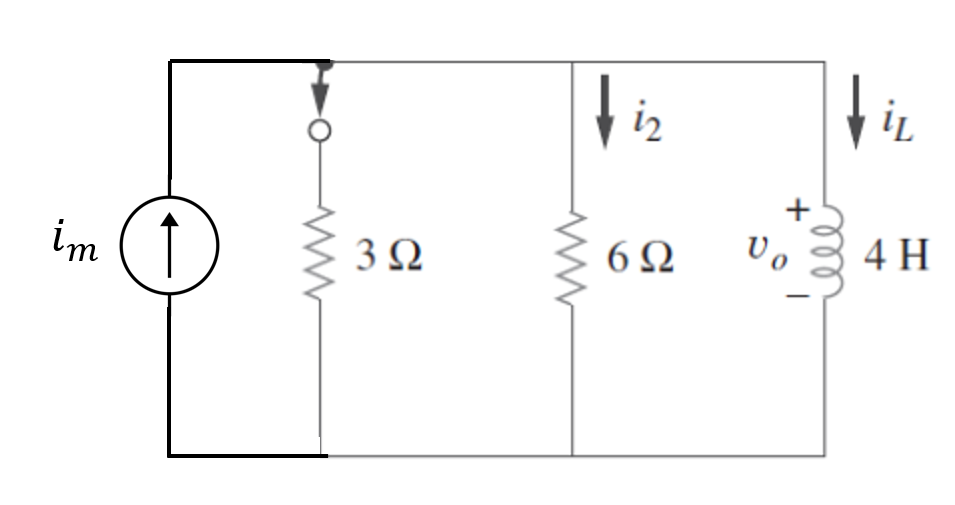
\includegraphics[width=0.6\textwidth]{Auxiliar_5_8}
            \captionof{figure}{Esquema del circuito para un tiempo $t>0$}
        \end{center}
        Luego tendremos que el sistema de ecuaciones sera el siguiente:
        \begin{align}
            \frac{V_{0}}{3} + \frac{V_{0}}{6} + i_{l} - i_{m} &= 0\\
            \frac{V_{0}}{2} + i_{l} &= i_{m}
        \end{align}
        Donde tenemos que el voltaje $V_{0} = L \frac{\partial i_{l}}{\partial t}$ y la corriente $i_{m} = e^{-\frac{1}{2}t}$, por lo que tenemos que:
        \begin{align}
            \frac{L}{2} \frac{\partial i_{l}}{\partial t} + i_{L} = e^{-\frac{1}{2}t}\\
            \frac{\partial i_{l}}{\partial t} + \frac{2}{L} i_{L} = \frac{2}{L} e^{-\frac{1}{2}t}
        \end{align}
        Dado que estamos en el caso de la RENC, luego tendremos que considerar la condicion inicial nula $i_{l}(t=0) = 0$ y por lo tanto tenemos que la respuesta sera:
        \begin{align}
            i_{l}= \frac{1}{2}te^{-\frac{1}{2}t}
        \end{align}
        Luego se pide obtener la RENC, por lo que se consideran las fuentes de voltaje/corrientes apagadas y se deben considerar las condiciones iniciales, por lo que el circuito vendra dado por:
        \begin{center}
            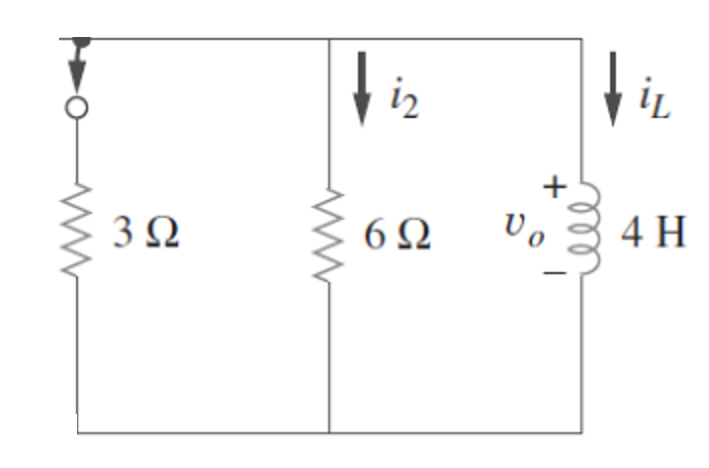
\includegraphics[width=0.4\textwidth]{Auxiliar_5_9}
            \captionof{figure}{Esquema del circuito para un tiempo $t>0$}
        \end{center}
        Con lo que tendremos que el sistema de ecuaciones sera:
        \begin{align}
            \frac{V_{0}}{3} + \frac{V_{0}}{6} + i_{l} &= 0\\
            \frac{V_{0}}{2} + i_{l} &= 0\\
            \frac{\partial i_{l}}{\partial t} + \frac{2}{L}i_{l} = 0
        \end{align}
        Considerando que $i_{l}(t=0) = 3[A]$, tenemos que la respuesta RENC vendra dada por:
        \begin{align}
            i_{l}(t) = 3 \cdot e^{-\frac{1}{2}t}
        \end{align}
        \item Luego tenemos que la respuesta completa vendra dada por:
        \begin{align}
            i_{L}(t) = 3\cdot e^{-\frac{1}{2}t} + \frac{1}{2}te^{-\frac{1}{2}t}
        \end{align}
         para todo $t > 0 $
    \item Se busca analizar la situacion cuando $i_{L}(t \to \infty)$, por lo que tenemos que:
    \begin{align}
        i_{L}(\infty) = 3\cdot e^{-\frac{1}{2}\infty} + \frac{1}{2}\infty e^{-\frac{1}{2}\infty}\\
        i_{L}(\infty) = 0 + 0 = 0
    \end{align}
    Tenemos algo con sentido dado que la fuente de corriente a la cual esta conectada tiende a 0, por lo que la corriente por la inductancia tiende a 0.
    \item Para la sexta pregunta, se está pidiendo el valor de \( i_1(t) \), \( i_2(t) \) y \( V_0(t) \) cuando \( t \to \infty \).Por la explicación anterior, todos los parámetros de corrientes se van a cero excepto \( i_1(t) \), ya que tal corriente circula por el circuito desacoplado de la izquierda. Por lo tanto:
    \begin{align}
    i_1(t \to \infty) &= 2\,[\text{A}] \\
    i_2(t \to \infty) &= 0\,[\text{A}] \\
    V_0(t \to \infty) &= 0\,[\text{A}]
    \end{align}
    \end{enumerate}
\end{solution}
    %%%%%%%%%%%%%%%%%%%%%%%%%%%%
    \question
    Para la red de la figura que está en régimen permanente con el interruptor conectado a la fuente de 20\,[V], en \( t = 0 \) se cambia el interruptor a la fuente \( v_s(t) \). Si \( v_s(t) = 4 \) para \( t \geq 0 \), determine:

\begin{enumerate}
    \item La respuesta de Entrada Cero.
    \item La respuesta de Estado Cero.
    \item La respuesta completa, identificando su parte permanente y su parte transitoria.
    \item \textbf{Propuesto:} Analice qué tipo de gráfico es (subamortiguado, amortiguado, sin pérdidas, etc.).
\end{enumerate}
\begin{center}
    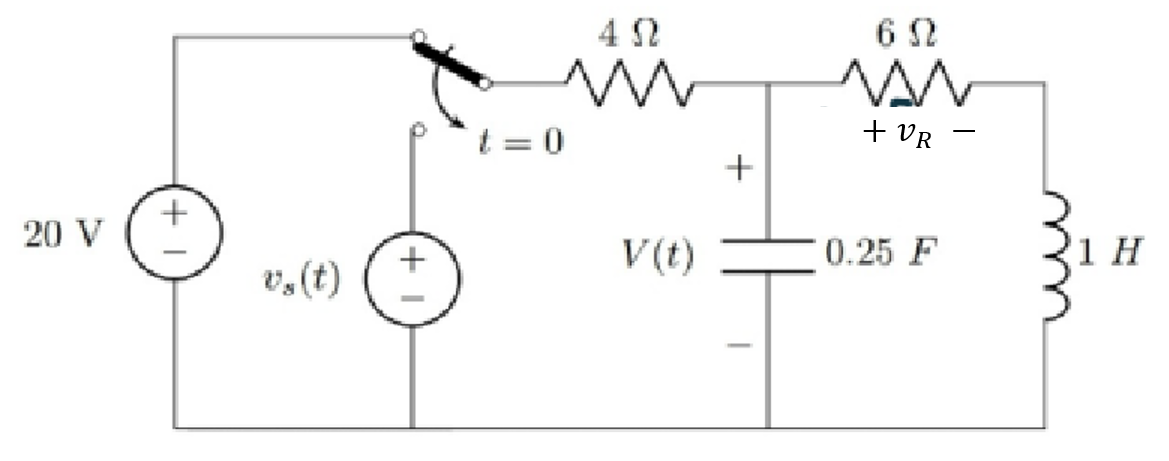
\includegraphics[width=0.6\textwidth]{Auxiliar_5_11}
    \captionof{figure}{Esquema del circuito}
\end{center}

Todo esto para la resistencia \(V_R(t)\).
%%%%%%%%%%%%%%%%%%%%%%%%%%%%%%
\begin{solution}
    \begin{enumerate}
        \item Se busca obtener la RENC, por lo que tenemos el siguiente esquema:
        \begin{center}
            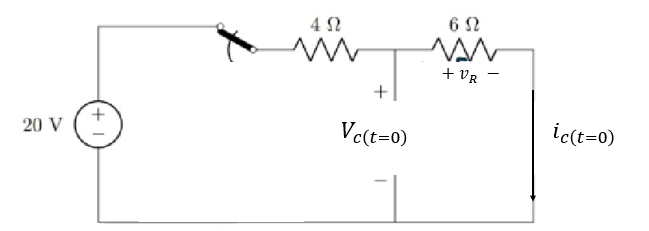
\includegraphics[width=0.6\textwidth]{Auxiliar_5_12}
            \captionof{figure}{Esquema del circuito para un tiempo $t<0$}
        \end{center}
        Tenemos que las inductancia se comportara como un cortocircuito, mientras que el condensador se comportara como un circuito abierto, esto para un tiempo infinitamente largo. Realizando una malla tenemos que:
        \begin{align}
            -20 + 4i_{l} + 6i_{l} &= 0\\
            i_{l} &= 2[A]
        \end{align}
        De esta manera tenemos que la corriente de la inductancia sera $i_{l}(t<0)= 2[A]$ mientras que el voltaje del condensador esta en paralelo con la resistencia $V_{R}$ por lo que:
        \begin{align}
            V_{c} = V_{R} = 6 \cdot 2 = 12[V]
        \end{align}
        Asi tenemos que el voltaje del condensador sera $V_{c}(t<0)=12[V]$. Luego para el cambio de Switch tenemos que el circuito sera el siguiente:
        \begin{center}
            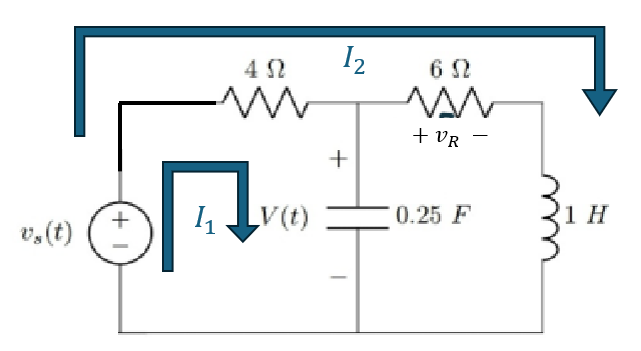
\includegraphics[width=0.6\textwidth]{Auxiliar_5_13}
            \captionof{figure}{Esquema del circuito para un tiempo $t>0$}
        \end{center}
        De esta manera tenemos que la malla 1 vendra dada por:
        \begin{align}
            -v_{s} + 4(i_{1}+i_{2}) + v_{c} &= 0\\
            4(i_{1}+i_{2}) + v_{c} &=  v_{s}\\
        \end{align}
        Dado que el voltaje en el condensador es $v_{c} = \frac{1}{C} \int i(t) \partial t$, por lo que siempre es conveniente derivar este tipo de expresiones para no trabajar con la integral, asi tenemos que:
        \begin{align}
            4(i_{1}^{'}+i_{2}^{'}) + \frac{1}{C} i_{1} &=  v_{s}^{'}\\
        \end{align}
        Luego tenemos que la malla 2 correspondera a:
        \begin{align}
            -v_{s} + 4(i_{1}+i_{2}) + 6i_{2} + v_{l}&= 0\\
            -v_{s} + 4(i_{1}+i_{2}) + 6i_{2} + L i_{2}^{'} &= 0\\
             4(i_{1}+i_{2}) + 6i_{2} + L i_{2}^{'} &= v_{s}\\
        \end{align}
        Luego podemos igualar las ecuaciones de la malla 1 y 2, pero para esto devemos derivar esta ultima ecuacion, por tanto:
        \begin{align}
            4(i_{1}^{'}+i_{2}^{'}) + 6i_{2}^{'} + L i_{2}^{''} &= v_{s}^{'}\\
        \end{align}
        Con lo que de esta manera:
        \begin{align}
            4(i_{1}^{'}+i_{2}^{'}) + 6i_{2}^{'} + L i_{2}^{''} &= 4(i_{1}^{'}+i_{2}^{'}) + \frac{1}{C} i_{1}
        \end{align}
        Luego reemplazando $L=1[H]$ y $C=0.25[F]$, tenemos que:
        \begin{align}
            \frac{3}{2}i_{2}^{'}+ \frac{1}{4}i_{2}^{''} = i_{1}
        \end{align}
        Se derivo las ecuaciones generales, dado que ahora buscamos la RENC, se impone que $v_{s} = 0$ por tanto tenemos que:
        \begin{align}
            4(i_{1} + i_{2}) + 6i_{2} + L i_{2}^{'} &= v_{s}\\\
            4(i_{1} + i_{2}) + 6i_{2} + L i_{2}^{'} &= 0\\
        \end{align}
        Luego se reemplaza $i_{1} = \frac{3}{2}i_{2}^{'}+ \frac{1}{4}i_{2}^{''}$, por lo que tenemos que:
        \begin{align}
            4\left(\frac{3}{2}i_{2}^{'}+ \frac{1}{4}i_{2}^{''} + i_{2}\right) + 6i_{2} + L i_{2}^{'} &= 0
        \end{align}
        Reeorganizando la ecuacion tenemos que:
        \begin{align}
            i_{2}^{''} + 7i_{2}^{'} + 10i_{2} &= 0\\
        \end{align}
        Nos falta una condicion inicial para $i_{2}^{'}(t=0)$, se puede derivar de:
        \begin{align}
            V_{c}(t=0) &= V_{L}(t=0) + V_{R}(t=0)\\
            12 &= L \cdot I_{2}^{'} + 6 \cdot 2\\
            12 &= L \cdot I_{2}^{'} + 12\\
            0 &= L \cdot I_{2}^{'}\\
            I_{2}^{'}(t=0) &= 0
        \end{align}
        Con lo que se obtiene la condicion inicial faltante, de esta manera tenemos finalmente que la respuesta sera:
        \begin{align}
            i_{2}(t) = \frac{10}{3}e^{-2t}
        \end{align}
        De esta manera tenemos que el voltaje en la resistencia para la respeusta RENC sera:
        \begin{align}
            V_{R}(t) = 6 \cdot i_{2}(t) = 20e^{-2t} - 8e^{-5t}
        \end{align}
        \item  Se busca obtener la RESC, por lo que consideramos que las fuentes estan encendidas pero con condiciones iniciales nulas ($i_{2}(t=0) = 0$ y $i_{2}^{'}(t=0)=0$), por lo tanto retomando las ecuaciones anteriores:
        \begin{align}
            i_{2}^{''} + 7i_{2}^{'} + 10i_{2} &= v_{s}\\
            i_{2}^{''} + 7i_{2}^{'} + 10i_{2} &= 4\\
        \end{align}
        Por lo que resolviendo la ecuacion diferencial tenemos que:
        \begin{align}
            V_{R}(t) = -4e^{-2t} + \frac{24}{15}e^{-5t} + \frac{12}{5}
        \end{align}
        Por lo que se obtiene la RESC
        \item La respuesta completa vendra dada por la suma de la RENC y RESC, por lo que tenemos que:
        \begin{align}
            V_{R}(t) = 20e^{-2t} - 8e^{-5t} -4e^{-2t} + \frac{24}{15}e^{-5t} + \frac{12}{5}\\
            V_{R}(t) = 16e^{-2t} - \frac{32}{5}e^{-5t} + \frac{12}{5}
        \end{align}
        Donde se identifica que la parte transitoria sera $16e^{-2t} - \frac{32}{5}e^{-5t}$ y la parte permanente sera $\frac{12}{5}$. Esto se entiende como que la parte transitoria tiende a cero cuando $t \to \infty$, mientras que la parte permanente se mantiene constante sin importar el tiempo.
    \end{enumerate}
\end{solution}
%%%%%%%%%%%%%%%%%%%%%%%%%%%%%%:
\end{questions}

\end{document}